% =====================================================================
%  SMILify — Internship Presentation (15 minutes)
%  Joint-Limit Regularization under Single- and Multi-View Supervision
%
%  Design system
%    type      Lato (humanist sans), graceful fallback if unavailable
%    palette   warm paper + ink, two accents only:
%                teal  = single-view / improvement
%                coral = multi-view  / cost
%    figures   drawn natively (TikZ/pgfplots) from the study numbers,
%              so every chart shares the deck's palette
%
%  Compile: pdflatex twice (no shell-escape needed).
%  Figures expected in ./fig/
% =====================================================================
\documentclass[aspectratio=169,11pt]{beamer}

% ---------- theme (with fallback so this always compiles) ------------
\IfFileExists{beamerthememetropolis.sty}{%
  \usetheme[progressbar=none,numbering=none,block=fill,sectionpage=none]{metropolis}%
}{%
  \usetheme{default}\usefonttheme{professionalfonts}%
}

\usepackage[T1]{fontenc}
\usepackage[utf8]{inputenc}
\IfFileExists{lato.sty}{\usepackage[defaultsans]{lato}}{}
\IfFileExists{inconsolata.sty}{\usepackage[scaled=0.92]{inconsolata}}{}
\renewcommand{\familydefault}{\sfdefault}

% report figures are used in place; nothing is copied into fig/
\graphicspath{{fig/}{../../report_joint_limit_prior/figures/}}
\usepackage{booktabs}
\usepackage{array}
\usepackage{amsmath}
\usepackage{tikz}
\usepackage{pgfplots}
\pgfplotsset{compat=1.17}
\usetikzlibrary{arrows.meta,positioning,fadings,calc,shapes.geometric}
\usepackage{xcolor}

% =====================================================================
%  PALETTE  — two accents, warm neutrals. Nothing else.
% =====================================================================
\definecolor{ink}    {HTML}{1E2430}   % primary text
\definecolor{inkSoft}{HTML}{4A5260}   % secondary text
\definecolor{muted}  {HTML}{9A968F}   % tertiary / placeholders
\definecolor{paper}  {HTML}{FAF7F4}   % background
\definecolor{hair}   {HTML}{E4DDD5}   % hairlines
\definecolor{teal}   {HTML}{0F6F68}   % accent 1 — single-view / better
\definecolor{tealLt} {HTML}{D7E8E5}
\definecolor{coral}  {HTML}{C85A44}   % accent 2 — multi-view / cost
\definecolor{coralLt}{HTML}{F5E1DB}

\setbeamercolor{normal text}{fg=ink,bg=paper}
\setbeamercolor{background canvas}{bg=paper}
\setbeamercolor{frametitle}{fg=ink,bg=paper}
\setbeamercolor{title}{fg=ink}
\setbeamercolor{alerted text}{fg=teal}
\setbeamercolor{itemize item}{fg=teal}
\setbeamercolor{itemize subitem}{fg=muted}
\setbeamercolor{enumerate item}{fg=teal}
\setbeamercolor{block title}{fg=ink,bg=hair!45}
\setbeamercolor{block body}{fg=inkSoft,bg=hair!20}
\setbeamercolor{block title alerted}{fg=white,bg=teal}
\setbeamercolor{block body alerted}{fg=ink,bg=tealLt}
\setbeamercolor{block title example}{fg=white,bg=coral}
\setbeamercolor{block body example}{fg=ink,bg=coralLt}

\setbeamerfont{frametitle}{size=\large,series=\bfseries}
\setbeamerfont{title}{size=\Huge,series=\bfseries}
\setbeamerfont{block title}{size=\small,series=\bfseries}
\setbeamerfont{block body}{size=\small}
\setbeamertemplate{itemize items}{\color{teal}\raisebox{0.12ex}{\scriptsize$\bullet$}}
\setbeamertemplate{navigation symbols}{}

% ---- frame title: ink on paper + hairline, no heavy bars ------------
\setbeamertemplate{frametitle}{%
  \nointerlineskip\vskip0.72em%
  \begin{beamercolorbox}[wd=\paperwidth,leftskip=1.2em,rightskip=1.2em]{frametitle}%
    \usebeamerfont{frametitle}\insertframetitle\par\vskip0.35em%
    {\color{teal}\rule{2.2em}{1.6pt}}\hspace{-0.35em}%

  \end{beamercolorbox}\vskip0.42em%
}

% ---- discreet footer: section · slide number -------------------------
\setbeamertemplate{footline}{%
  \hbox{\begin{beamercolorbox}[wd=\paperwidth,ht=2.2ex,dp=1.4ex,
      leftskip=1.2em,rightskip=1.2em]{}%
    {\color{muted}\scriptsize\insertsection\ \ $\cdot$\ \ \insertframenumber}%
    \hfill
    \raisebox{0.10cm}[0pt][0pt]{\fzjlogo}%
  \end{beamercolorbox}}%
}

% =====================================================================
%  MICRO-COMPONENTS — the deck's visual vocabulary
% =====================================================================
% delta chip: \chip{teal}{-55}
\newcommand{\chip}[2]{%
  \tikz[baseline=(x.base)]{\node[inner xsep=4pt,inner ysep=1.6pt,
    rounded corners=2pt, fill=#1!12, text=#1!85!black,
    font=\footnotesize\bfseries] (x) {#2};}}
\newcommand{\gain}[1]{\chip{teal}{$\downarrow$\,#1}}
\newcommand{\cost}[1]{\chip{coral}{$\uparrow$\,#1}}
\newcommand{\ph}[1]{{\color{muted}\itshape #1}}
% sweep-table helpers
\newcommand{\ctrlrow}[1]{{\color{inkSoft}#1}}
\newcommand{\hd}[1]{{\color{inkSoft}\scriptsize\bfseries #1}}

% big stat: \stat{96}{violating axes}
\newcommand{\stat}[3]{%
  \begin{minipage}[t]{#1}\raggedright
    {\color{teal}\fontsize{22}{24}\selectfont\bfseries #2}\\[0.15em]
    {\color{inkSoft}\scriptsize #3}
  \end{minipage}}

% before -> after bar, scaled to 162 axes
\newcommand{\axisbar}[3]{% #1 colour #2 before #3 after
  \begin{tikzpicture}[x=0.030\textwidth,y=1ex]
    \fill[hair!60]      (0,0) rectangle (#2*0.16,1.5);
    \fill[#1]           (0,0) rectangle (#3*0.16,1.5);
  \end{tikzpicture}}

% Forschungszentrum Julich mark — white keyed out, sits on any ground
\newcommand{\fzjlogo}[1][1.45cm]{\includegraphics[width=#1]{fig/fzj_logo_trim.png}}

% section divider
\newcommand{\sectionslide}[3]{%
\begin{frame}[plain]
  \begin{tikzpicture}[remember picture,overlay]
    \fill[paper] (current page.south west) rectangle (current page.north east);
    \draw[teal,line width=1.6pt]
      ($(current page.west)+(1.4cm,2.15cm)$) -- ++(2.2cm,0);
    \node[anchor=north west, text width=0.72\paperwidth]
      at ($(current page.west)+(1.4cm,1.75cm)$) {%
      {\color{teal}\fontsize{40}{42}\selectfont\bfseries #1}\\[0.45em]
      {\color{ink}\fontsize{22}{26}\selectfont\bfseries #2}%
      \ifx\relax#3\relax\else\\[0.55em]{\color{inkSoft}\small #3}\fi};
    \node[anchor=south east, inner sep=0]
      at ($(current page.south east)+(-1.2cm,0.62cm)$) {\fzjlogo};
  \end{tikzpicture}
\end{frame}}

% ---- pgfplots house style -------------------------------------------
\pgfplotsset{
  house/.style={
    font=\scriptsize,
    axis line style={hair!90, line width=0.6pt},
    tick style={hair!90, line width=0.6pt},
    label style={inkSoft, font=\scriptsize},
    tick label style={inkSoft, font=\scriptsize},
    title style={ink, font=\small\bfseries, yshift=2pt},
    legend style={draw=none, fill=none, font=\scriptsize, text=inkSoft},
    grid style={hair!70, line width=0.4pt},
    axis background/.style={fill=paper},
  }
}

% =====================================================================
\begin{document}
\setbeamercolor{background canvas}{bg=paper}

% ---------------------------------------------------------------------
%  TITLE — institutional plate (carries the Julich mark itself)
% ---------------------------------------------------------------------
\begin{frame}[plain]
\begin{tikzpicture}[remember picture,overlay]
  \node[anchor=south west, inner sep=0] at (current page.south west)
    {
\includegraphics[width=\paperwidth,height=\paperheight]{fig/image.png}};

  % all type stays inside the bright left third of the plate
  \node[anchor=north west, text width=0.42\paperwidth, inner sep=0]
    at ($(current page.north west)+(1.35cm,-0.95cm)$) {%
      {\color{teal}\scriptsize\bfseries INTERNSHIP DEFENCE}\\[0.22em]
      {\color{muted}\scriptsize FZJ, IAS-7}\\[0.85em]
      {\color{ink}\fontsize{32}{34}\selectfont\bfseries SMILify}\\[0.45em]
      {\color{inkSoft}\fontsize{11.5}{14.5}\selectfont
        \hyphenpenalty=10000 \exhyphenpenalty=10000 \sloppy
        Refactoring and Extending Parametric 3D Modelling Across Species}\\[0.8em]
      {\color{teal}\rule{2.4cm}{1.5pt}}\\[0.65em]
      {\color{ink}\small Youness Anouar}\\[0.22em]
      {\color{muted}\footnotesize Supervisor: Fabian Plum \ $\cdot$ \ 21 sep 2026}};
\end{tikzpicture}
\end{frame}

% ---------------------------------------------------------------------
\begin{frame}{The talk in one slide}
  \vspace{0.2em}
  \begin{columns}[T,onlytextwidth]
    \column{0.305\textwidth}
      {\color{teal}\footnotesize\bfseries 01 \ THE GAP}\\[0.45em]
      {\small Parametric 3D models exist for humans and quadrupeds.
      SMILify opens them to \textbf{any rigged species}, but its fits
      are anatomically under-constrained.}
    \column{0.305\textwidth}
      {\color{teal}\footnotesize\bfseries 02 \ THE WORK}\\[0.45em]
      {\small I stabilized the pipeline, then encoded
      \textbf{162 joint limits} from stick-insect biomechanics as a
      differentiable penalty.}
    \column{0.305\textwidth}
      {\color{teal}\footnotesize\bfseries 03 \ THE QUESTION}\\[0.45em]
      {\small Do anatomical priors help equally when the cameras
      already tell you the answer? \textbf{Single-view vs.\
      multi-view.}}
  \end{columns}
  \vspace{1.1em}

  \vspace{0.3em}


\end{frame}

% =====================================================================
\section{Context}
\sectionslide{01}{Context and motivation}{From human body models to a body-plan-agnostic toolset}


% ============================================================
% SLIDE 1 — SMILify for non-experts
% ============================================================
\begin{frame}{SMILify: Building 3D body models from images}

\begin{itemize}
    \item SMPL: parametric 3D human body model
    \item SMILify: like SMPL, but for any body plan
\end{itemize}

\centering
\includegraphics[
    width=\textwidth,
    height=0.65\textheight,
    keepaspectratio
]{fig/algo_side2.png}

\end{frame}

\begin{frame}{SMILify: Building 3D body models from images}
    Images → NN → (Shape $\beta$, Pose $\theta$, camera $\gamma$) → SMAL/SMIL model → 3D mesh
\begin{itemize}
    \item Body-plan agnostic workflow for building parametric models
    \item Designed to transfer across different species / morphologies
    \item Focus: how to build models, rather than one specific body model
\end{itemize}



\end{frame}
\begin{frame}{Back to pedestrian dynamics}
    \begin{enumerate}
        \item Inference: 
        \begin{itemize}
            \item Fused computer vision + X-sense mocap
            \item Extract movement patterns

        \end{itemize}
        \item Analysis:
        \begin{itemize}
            \item Contacts & collisions → force propagation
            \item Body attributes → visibility / interaction analysis
        \end{itemize}
    \end{enumerate}
\end{frame}


\begin{frame}{Two problems}
  \vspace{0.3em}
  \begin{columns}[T,onlytextwidth]
    \column{0.47\textwidth}
      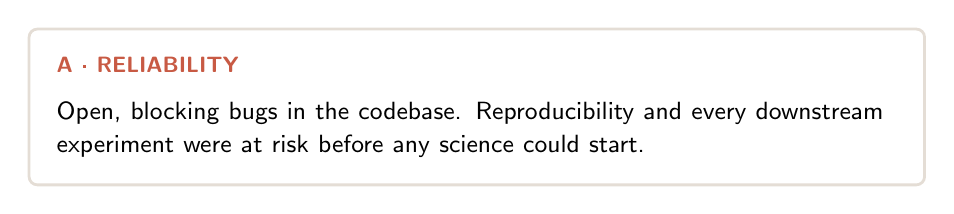
\begin{tikzpicture}
        \node[draw=hair, line width=1pt, fill=white, rounded corners=3pt,
          inner sep=10pt, text width=0.88\textwidth, align=left] {%
          {\color{coral}\footnotesize\bfseries A · RELIABILITY}\\[0.5em]
          {\small Open, blocking bugs in the codebase. Reproducibility
          and every downstream experiment were at risk before any
          science could start.}};
      \end{tikzpicture}
    \column{0.47\textwidth}
      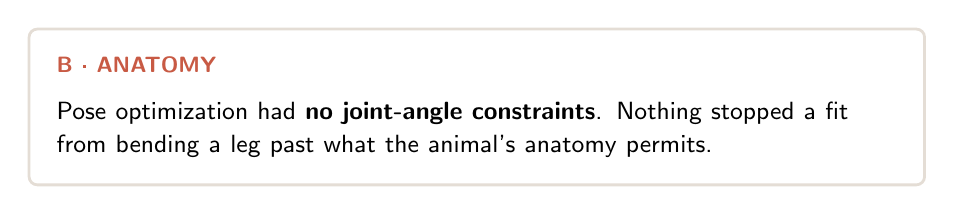
\begin{tikzpicture}
        \node[draw=hair, line width=1pt, fill=white, rounded corners=3pt,
          inner sep=10pt, text width=0.88\textwidth, align=left] {%
          {\color{coral}\footnotesize\bfseries B · ANATOMY}\\[0.5em]
          {\small Pose optimization had \textbf{no joint-angle
          constraints}. Nothing stopped a fit from bending a leg past
          what the animal's anatomy permits.}};
      \end{tikzpicture}
  \end{columns}
  \vspace{1.3em}
  \begin{alertblock}{The question this internship asks}
    Does enforcing biomechanically-grounded joint limits improve
    reconstruction, and does the answer change between single-view
    and multi-view supervision?
  \end{alertblock}
\end{frame}

\begin{frame}{Objectives}
  \vspace{0.5em}
  \begin{columns}[T,onlytextwidth]
    \column{0.06\textwidth}
      {\color{teal}\small\bfseries 1\\[1.15em] 2\\[1.15em] 3\\[1.15em] 4\\[1.15em] 5}
    \column{0.9\textwidth}
      {\small Stabilize the codebase}\\[0.75em]
      {\small Curate anatomically valid joint limits from the literature}\\[0.75em]
      {\small Quantify the effect of the prior on \textbf{single-view} fitting}\\[0.75em]
      {\small Quantify the effect of the prior on \textbf{multi-view} fitting}\\[0.75em]
    {\small Quantify the effect of the prior on 2D (only) supervised \textbf{single-view} fitting}
  \end{columns}
  \vspace{1.2em}

\end{frame}

% =====================================================================
\section{Engineering}
\sectionslide{02}{The engineering foundation}{}

\begin{frame}{Stabilizing the pipeline}
  \vspace{0.35em}
  {\footnotesize
  \renewcommand{\arraystretch}{1.02}%
  \begin{tabular}{@{}p{0.85cm} >{\raggedright\arraybackslash}p{4.9cm}
                    >{\raggedright\arraybackslash}p{6.7cm}@{}}
    \toprule
    {\color{inkSoft}\scriptsize\bfseries ISSUE} &
    {\color{inkSoft}\scriptsize\bfseries FIX} &
    {\color{inkSoft}\scriptsize\bfseries WHY IT MATTERED} \\
    \midrule
    \textbf{\#24}  & \texttt{pose\_dirs} repaired for legacy,
      non-human rigs & Correct mesh registration under every later
      fit \\[0.4em]
    \textbf{\#25}  & A 4\,000-line script refactored into an
      installable add-on & Maintainable, reproducible rig
      preparation \\[0.4em]
    {\color{teal}\textbf{\#56}}  & Per-joint rotation limits, authored
      and exported to the model file &
      {\color{teal}\textbf{Prerequisite for the prior}} — what makes
      literature limits usable \\[0.4em]
    {\color{teal}\textbf{\#100}} & Single-view inference aligned to the
      multi-view output format &
      {\color{teal}\textbf{Prerequisite for the comparison}} — SV and
      MV become directly comparable \\
    \bottomrule
  \end{tabular}}
  \vspace{0.75em}


\end{frame}

% =====================================================================
\section{Method}
\sectionslide{03}{Joint-limit regularization}

\begin{frame}{From published kinematics to per-axis limits}
  \begin{columns}[T,onlytextwidth]
    \column{0.5\textwidth}
      \textbf{\small Species:} {\small\emph{Carausius morosus}
      (Phasmatodea)}
      \begin{itemize}\setlength\itemsep{0.4em}
        \item {\small Leg and head ranges from three kinematics
          studies\,\footnotemark[1]
          }
        \item {\small Mapped onto the 55-joint rig (axis-angle, global
          frame)}
        \item {\small \textbf{162} non-root axes, each with a
          \((\theta^{\min},\theta^{\max})\) range:
          55 limited, 74 locked, 33 free}
      \end{itemize}

    \column{0.46\textwidth}
      \centering
      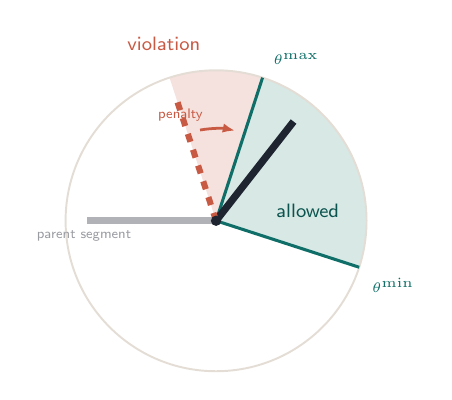
\begin{tikzpicture}[scale=0.78]
        \def\lo{-18} \def\hi{72} \def\ovr{108}
        % wedges
        \fill[tealLt]  (0,0) -- (\lo:2.45) arc (\lo:\hi:2.45) -- cycle;
        \fill[coral!18] (0,0) -- (\hi:2.45) arc (\hi:\ovr:2.45) -- cycle;
        \draw[hair, line width=0.7pt] (0,0) circle (2.45);
        % limit rays
        \draw[teal, line width=1.1pt] (0,0) -- (\lo:2.45);
        \draw[teal, line width=1.1pt] (0,0) -- (\hi:2.45);
        % proximal segment (fixed) and a valid pose
        \draw[ink!35, line width=2.6pt] (0,0) -- (180:2.1);
        \draw[ink, line width=2.6pt]    (0,0) -- (52:2.05);
        % violating pose
        \draw[coral, line width=2.2pt, dashed] (0,0) -- (\ovr:2.05);
        \fill[ink] (0,0) circle (2.4pt);
        % pull-back arrow
        \draw[-{Latex[length=4.5pt]}, coral, line width=1pt]
          (100:1.5) arc (100:78:1.5);
        % labels
        \node[teal, font=\tiny, anchor=north west] at (\lo:2.5) {$\theta^{\min}$};
        \node[teal, font=\tiny, anchor=south west] at (\hi:2.5) {$\theta^{\max}$};
        \node[teal!75!black, font=\scriptsize] at (6:1.5) {allowed};
        \node[coral, font=\scriptsize, anchor=south] at (\ovr:2.75) {violation};
        \node[coral, font=\tiny, anchor=east] at (92:1.72) {penalty};
        \node[ink!45, font=\tiny, anchor=north] at (180:2.15) {parent segment};
      \end{tikzpicture}
  \end{columns}
  \footnotetext[1]{\scriptsize Theunissen et al.\ (2015);
    Guschlbauer et al.\ (2022); Dallmann et al.\ (2016).}
\end{frame}
\begin{frame}{The augmented loss}
  \vspace{0.4em}
  Rotations outside their authored range are penalized linearly;
  everything inside the range costs nothing.
  \vspace{0.5em}
  \[
    \mathcal{L}_{\mathrm{JLR}}=\frac{1}{N\,|A|}\sum_{n=1}^{N}\sum_{a\in A}
      \Big[\max\!\big(0,\;\theta_{n,a}-\theta_a^{\max}\big)
         + \max\!\big(0,\;\theta_a^{\min}-\theta_{n,a}\big)\Big]
    \qquad
    \mathcal{L}_{\text{total}}=\mathcal{L}_{\text{fit}}
      +\lambda\,\mathcal{L}_{\mathrm{JLR}}
  \]
  \vspace{0.3em}
  \begin{columns}[T,onlytextwidth]
    \column{0.47\textwidth}
      \begin{itemize}\setlength\itemsep{0.35em}
        \item {\small $\theta_{n,a}$: axis-angle component $a$ of sample $n$}
        \item {\small $A$: the 162 rotation axes; $N$: valid samples in the batch}

      \end{itemize}
  \end{columns}
\end{frame}

% =====================================================================
\section{Results}
\sectionslide{04}{Experiments and results}

\begin{frame}{Two experiments, different questions}
\begin{enumerate}

    \item Does adding an authored per-joint rotation prior to the neural stick-insect model produce more anatomically plausible poses without losing 3D and 2D accuracy?
    \item Does adding an authored per-joint rotation prior to the neural stick-insect model help infer 3D information from 2D-only supervision?
\end{enumerate}    
\end{frame}
\begin{frame}{Dataset}
  \vspace{0.2em}

  % Dataset overview
  \begin{block}{\centering \textbf{SMILySTICKS} — Multi-view stick-insect dataset}
    \centering
    5 calibrated cameras \quad $\cdot$ \quad
    55 joints \quad $\cdot$ \quad
    5 synchronized views \quad $\cdot$ \quad
    6 different stick insect species 
  \end{block}

  \vspace{0.7em}

  \begin{columns}[T,onlytextwidth]

    % Left: dataset split
    \column{0.48\textwidth}
    {\color{teal}\footnotesize\bfseries DATA SPLIT}

    \vspace{0.35em}

    \begin{tabular}{@{}lr@{}}
      Train & 86\,062 frames \\
      Validation & 5\,062 frames \\
      \textbf{Test} & \textbf{10\,126 frames}
    \end{tabular}

    \vspace{0.3em}

    {\footnotesize\color{inkSoft}
    Each frame contains up to 5 synchronized camera views.}

    % Right: evaluation units
    \column{0.48\textwidth}
    {\color{teal}\footnotesize\bfseries EVALUATION}

    \vspace{0.35em}

    \begin{tabular}{@{}ll@{}}
      \textbf{Single-view (SV)} & 1 view / item \\
      \textbf{Multi-view (MV)} & 5 views / item
    \end{tabular}

    \vspace{0.3em}

    {\footnotesize\color{inkSoft}
    SV test set: $10\,126 \times 5 = 50\,630$ view-level items}

  \end{columns}

  \vspace{0.8em}

  % Conceptual distinction
  \begin{center}
    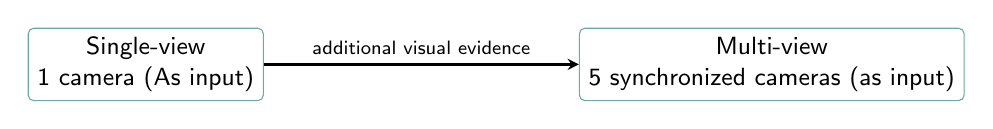
\begin{tikzpicture}[
      box/.style={
        draw=teal!60, rounded corners=2pt,
        minimum height=0.75cm, minimum width=2.5cm,
        align=center, font=\small
      },
      arrow/.style={->, thick, >=stealth}
    ]
      \node[box] (sv) {Single-view\\1 camera (As input)};
      \node[box, right=4cm of sv] (mv) {Multi-view\\5 synchronized cameras (as input)};

      \draw[arrow] (sv) -- node[above,font=\scriptsize] {additional visual evidence} (mv);
    \end{tikzpicture}
  \end{center}

\end{frame}

\begin{frame}{Experiment 1}
  \textbf{Protocol} {\small (same design in both modes)}
  \begin{itemize}\setlength\itemsep{0.3em}
    \item {\small Start from an established checkpoint, continue with
      identical schedule,  only \(\lambda\) differs}
      \begin{itemize}
        \item {\small \(\lambda = 0\): \textbf{epoch-matched control}
          (no prior), all comparisons are made against it}
        \item {\small \(\lambda \in \{10^{-4}, 10^{-3}, 10^{-2}, 10^{-1}\}\):
          fit loss \(+\,\lambda\,\mathcal{L}_{\mathrm{JLR}}\)}
      \end{itemize}
    \item {\small Same data, split and authored limits in both modes:
      SMILySTICKS, 10\,126 test samples}
  \end{itemize}

  \textbf{Metrics}
  \begin{itemize}\setlength\itemsep{0.2em}
    \item {\small \emph{Plausibility}: violation rate (\% of frames out of
      range), overshoot (\(^\circ\))}
    \item {\small \emph{Accuracy}: MPJPE (mm), PCK@5\,px, mean 2D error (px)}
    \item {\small \emph{Range of motion}: observed range per bounded axis
      vs.\ authored range}
  \end{itemize}
\end{frame}
% ---------------- single view ----------------------------------------
\begin{frame}{Results: Single-view vs. Multi-view}
        \centering
        
\includegraphics[
            width=\textwidth,
            height=0.52\textheight,
            keepaspectratio
        ]{figures/fig_mv_sv_compare.png}

    \begin{columns}[T,onlytextwidth]
    
        % --- LEFT: FIGURE ---
        \column{0.30\textwidth}
        \small
        \vspace{0.25em}
        \textbf{\color{teal}1. Joint limits work}
         
        Increasing $\lambda$ strongly reduces joint-limit violations
        for both models.
        % --- RIGHT: TAKEAWAYS ---
        \column{0.30\textwidth}
        \small
        \textbf{\color{teal}2. Accuracy–constraint trade-off}
        Stronger regularization comes at a cost:
        MPJPE increases as $\lambda$ increases.

        \column{0.30\textwidth}
        \small
        \textbf{\color{teal}3. Multi-view gives little extra 3D accuracy}
        At $\lambda=0$, both models achieve almost identical
        MPJPE ($\approx0.90$ mm).
        

        \vspace{0.8em}
        \textbf{\color{teal}Interpretation}
        
        \vspace{0.25em}
        With dense video sampling and strong 3D supervision,
        a single-view model already receives enough information
        to learn a strong 3D mapping.
    \end{columns}



\end{frame}
\begin{frame}{Range of motion: the prior removes more than violations}
  \begin{columns}[c,onlytextwidth]
    \column{0.6\textwidth}
    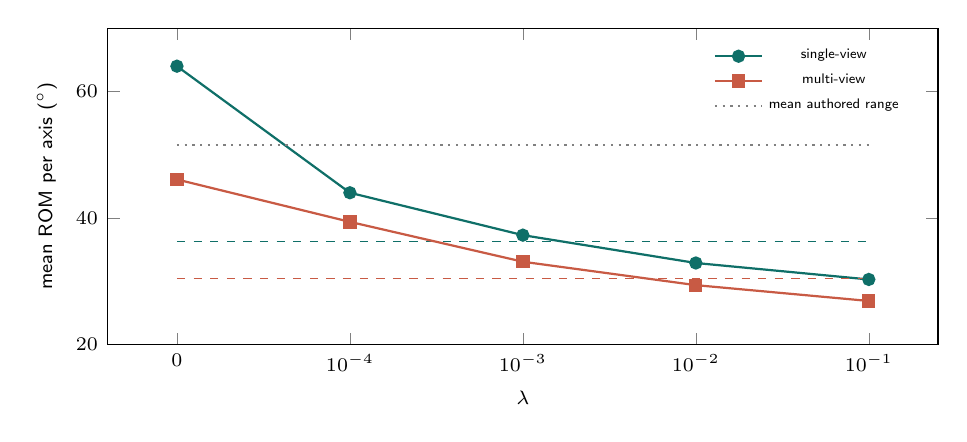
\begin{tikzpicture}
      \begin{axis}[
        width=\linewidth, height=5.6cm,
        symbolic x coords={0,1e-4,1e-3,1e-2,1e-1},
        xtick=data,
        xticklabels={$0$,$10^{-4}$,$10^{-3}$,$10^{-2}$,$10^{-1}$},
        xlabel={$\lambda$}, ylabel={mean ROM per axis ($^\circ$)},
        ymin=20, ymax=70,
        legend style={font=\tiny, draw=none, fill=none},
        legend pos=north east,
        tick label style={font=\scriptsize},
        label style={font=\scriptsize},
      ]
        % single-view
        \addplot[teal, thick, mark=*] coordinates
          {(0,64.0) (1e-4,44.0) (1e-3,37.3) (1e-2,32.9) (1e-1,30.3)};
        \addlegendentry{single-view}
        \addplot[teal, dashed, forget plot] coordinates {(0,36.3) (1e-1,36.3)};
        % multi-view
        \addplot[coral, thick, mark=square*] coordinates
          {(0,46.1) (1e-4,39.4) (1e-3,33.1) (1e-2,29.4) (1e-1,26.9)};
        \addlegendentry{multi-view}
        \addplot[coral, dashed, forget plot] coordinates {(0,30.5) (1e-1,30.5)};
        % authored range
        \addplot[gray, dotted, thick] coordinates {(0,51.6) (1e-1,51.6)};
        \addlegendentry{mean authored range}
      \end{axis}
    \end{tikzpicture}
    {\tiny Dashed: clipping bound (ROM left if the $\lambda{=}0$
    trajectory were only clipped into the authored range).}

    \column{0.37\textwidth}
    \begin{itemize}\setlength\itemsep{0.5em}
      \item {\small From $\lambda = 10^{-2}$ both modes drop
        \textbf{below} their clipping bound: joints stiffen where
        the penalty has no gradient}
      \item {\small Femur loses \textbf{73\,\%} (SV) /
        \textbf{72\,\%} (MV) of its range at $\lambda = 10^{-1}$}
      \item {\small MV starts inside the authored range
        ($46^\circ$ vs.\ $64^\circ$)}
    \end{itemize}
  \end{columns}
\end{frame}

\begin{frame}{Results: Demonstration}
 3 VIDEOS SITCK MOVING WITH PREDICTED MESH (exists) 
    
\end{frame}
\begin{frame}{Results: plot here on how the actual angles change over time}
    
\end{frame}

\begin{frame}{Results: Single-view vs. Multi-view}

\textbf{Main observation:}
The accuracy drop with increasing $\lambda$ is more pronounced for
multi-view than for single-view.

\vspace{0.7em}

\textbf{Possible interpretation:}

\begin{itemize}
    \item Multi-view provides stronger visual constraints, so its
    unconstrained solution may already be well determined.
    \item In single-view, the 3D pose is more ambiguous, so the joint-limit
    prior may help resolve some of this ambiguity.
\end{itemize}

\vspace{0.7em}

\textbf{This raises another question:}

\begin{center}
\itshape
Can authored per-joint rotation priors provide useful 3D information
when the single-view model is trained with only 2D supervision?
\end{center}

\vspace{0.4em}

\centering
$\rightarrow$ \textbf{Motivation for the next experiment}

\end{frame}



% ---------------- placeholder ----------------------------------------
\begin{frame}{Experiment 2:}
 \textbf{Protocol} {\small Single-view mode}
  \begin{itemize}\setlength\itemsep{0.3em}
    \item {\small Train from scratch with
      identical schedule,  only \(\lambda\) differs}
      \begin{itemize}
        \item {\small \(\lambda = 0\): 
          (no prior), all comparisons are made against it}
        \item {\small \(\lambda \in \{10^{-4}, 10^{-1}\}\):
          fit loss \(+\,\lambda\,\mathcal{L}_{\mathrm{JLR}}\)}
      \end{itemize}
    \item {\small Same data, split and authored limits in both modes:
      SMILySTICKS, 10\,126 test samples}
  \end{itemize}

  \textbf{Metrics}
  \begin{itemize}\setlength\itemsep{0.2em}
    \item {\small \emph{Plausibility}: violation rate (\% of frames out of
      range), overshoot (\(^\circ\))}
    \item {\small \emph{Accuracy}: MPJPE (mm), PCK@5\,px, mean 2D error (px)}
    \item {\small \emph{Range of motion}: observed range per bounded axis
      vs.\ authored range}
  \end{itemize}
\end{frame}


\begin{frame}{Results}
    
\end{frame}

\begin{frame}{Example SMILify outputs: Single-view and lambda=0 }
    VIDEO
\end{frame}

\begin{frame}{Example SMILify outputs: Single-view and lambda=1e-1 }
    VIDEO
\end{frame}

\section{Closing}

\sectionslide{05}{Discussion and outlook}{}

\begin{frame}{Discussion}

\end{frame}

\begin{frame}{Conclusion and outlook}
 
\end{frame}

% ---------------------------------------------------------------------
\begin{frame}[plain]
\begin{tikzpicture}[remember picture,overlay]
  \node[anchor=south west, inner sep=0] at (current page.south west)
    {
\includegraphics[width=\paperwidth,height=\paperheight]{fig/image.png}};
  \node[anchor=north west, text width=0.42\paperwidth, inner sep=0]
    at ($(current page.north west)+(1.35cm,-2.3cm)$) {%
      {\color{ink}\fontsize{30}{34}\selectfont\bfseries Thank you}\\[0.7em]
      {\color{teal}\rule{2.4cm}{1.5pt}}\\[0.85em]
      {\color{inkSoft}\large Questions?}\\[1.3em]
      {\color{muted}\footnotesize \texttt{Uness10/SMILify}\\[0.15em]
       fork of \texttt{FabianPlum/SMILify}}};
\end{tikzpicture}
\end{frame}

\end{document}
